\documentclass{beamer}
\usepackage[russian]{babel}
\usetheme{metropolis}

\usepackage{adjustbox}
\usepackage{makecell}

\usepackage{amsthm}
\setbeamertemplate{theorems}[numbered]

\setbeamercolor{block title}{use=structure,fg=white,bg=gray!75!black}
\setbeamercolor{block body}{use=structure,fg=black,bg=gray!20!white}

\usepackage[T2A]{fontenc}
\usepackage[utf8]{inputenc}

\usepackage{hyphenat}
\usepackage{amsmath}
\usepackage{graphicx}

\AtBeginEnvironment{proof}{\renewcommand{\qedsymbol}{}}{}{}

\title{
Микроэкономика-I
}
\author{
Павел Андреянов, PhD
}

\begin{document}

\maketitle

\section{План}

\begin{frame}{План}

Это пятая лекция.

В прошлом году я закончил теорию потребителя за 4 лекции.

В первой половине лекции мы поговорим о калибровке наших теоретических моделей поведения потребителей (30 слайдов).

Во второй половине лекции мы поговорим об эффектах дохода, замещения и разрешении парадокса Гиффена, что подведет к завершению наше изучение теории потребителя.

\end{frame}

\section{Калибровка}

\begin{frame}{Калибровка}

Экономисты часто занимаются \alert{калибровкой} - это процесс натягивания модели на данные, или наоборот. 

\begin{itemize}
  \item если мы танцуем от модели, то, грубо говоря $$ \alpha \log x + \beta \log y \text{ плюс данные} \to 3 \log x + 2 \log y$$
  \item если мы танцуем от данных, то можно получить бесплатно столбец данных которых у вас нет
  $$ \text{данные плюс структура модели} \to \text{больше данных}$$
... или лучше интерпретируемые данные
\end{itemize}

\end{frame}

\begin{frame}{Калибровка}

Например, я могу получить столбец предельных издержек ($mc$) из столбца цен ($p$), используя теоретическую структуру фирмы-монополиста ($(p - mc)/p = -1/\varepsilon$) или структуру фирмы-ценополучателя ($p = mc$).

Конечно, экономист должен решить сам, является ли фирма монополистом или нет, исходя из текстового описания задачи

\end{frame}

\begin{frame}{Калибровка}

Это, по сути, и есть основная роль экономиста, отличающая его от не-экономиста (дата аналиста, программиста, бухгалтера). 

\alert{Настоящий экономист} не программист и не бухгалтер, он немножко философ, он \alert{смотрит в суть вещей}.

\end{frame}

\begin{frame}{Калибровка}

Универсально доступны безразмерные метрики: доли (групп) товаров в расходах, всякие разные эластичности, изменения чего нибудь в процентах

Также доступны <<рублевые>> метрики: доход/расход, цены

Реже доступны <<штуковые>> метрики: расход электричества в ваттах, воды газа и бензина в литрах, количество автомобилей, детей, жен, и.т.п.

Чем проще размерность объекта тем проще его оценить. Максимально просты: дроби и проценты

\end{frame}

\section{Пример калибровки Леонтьева}

\begin{frame}{Леонтьев}

Рассмотрим полезность вида Леонтьев:
$$ U(x,y,z) = \min(x/a,y/b,z)$$
Как можно было бы откалибровать параметры $a$ и $b$?

\end{frame}

\begin{frame}{Леонтьев}

Вспомним спросы: 
$$ x^{\ast} = \frac{ap}{ap+bq+r}\frac{I}{p}, \quad y^{\ast} = \frac{bq}{ap+bq+r}\frac{I}{q}, \quad z^{\ast} = \frac{r}{ap+bq+r}\frac{I}{r}$$
Мы, конечно, наблюдаем спросы, но пока не очень понятно...
\end{frame}

\begin{frame}{Леонтьев}

Поделим все на $z^{\ast}$:
$$ x^{\ast}/z^{\ast} = a, \quad y^{\ast}/z^{\ast} = b$$
Заметим что отношение спросов не зависит от цен и бюджетов

В реальной жизни, конечно, же есть шум который не позволит этим соотношениям быть в точности константой...
\end{frame}

\begin{frame}{Леонтьев}

...но мы можем примерно оценить их
\begin{gather} \log x = \log z + \log a + \text{ошибка}\\ \quad \log y = \log z + \log b + \text{ошибка}\end{gather}
Это у экономистов называется <<гоним регрессию лог икс на лог зэт с константой>> и <<гоним регрессию лог y на лог зэт с константой>>, причем первый коэффициент регрессии мы ожидаем увидеть вблизи единички, иначе мы начнем сомневаться в правильности регрессии.

Подводя итог, полезность Леонтьева легко оценивается из отношения наблюдаемых спросов, в штуках. Кажется актуальным для потребления газа, электричества и воды и не сильно зависеть от размера домохозяйства.
\end{frame}

\section{Пример калибровки Кобб-Дугласа}

\begin{frame}{Кобб-Дуглас}

Рассмотрим полезность вида Кобб-Дуглас:
$$ U(x,y,z) = \alpha \log x + \beta \log y + \log z$$
Как можно было бы откалибровать параметры $\alpha$ и $\beta$?

\end{frame}

\begin{frame}{Кобб-Дуглас}

Вспомним спросы: 
$$ x^{\ast} = \frac{\alpha}{\alpha + \beta + 1}\frac{I}{p}, \quad y^{\ast} = \frac{\beta}{\alpha + \beta + 1}\frac{I}{q}, \quad z^{\ast} = \frac{1}{\alpha + \beta + 1}\frac{I}{r}$$
А что можно сделать тут?
\end{frame}

\begin{frame}{Кобб-Дуглас}
Рассмостим отношение расходов:
$$ px^{\ast}/rz^{\ast} = \alpha, \quad qy^{\ast}/rz^{\ast} = \beta$$
Заметим что оно не зависит от цен и бюджетов.

Причем данные по расходам <<в рублях>> гораздо проще получить чем данные по расходам <<в штуках>>.

\end{frame}

\begin{frame}{Кобб-Дуглас}
Врубаем режим экономиста
\begin{gather} \log x = \log \alpha + \log z + \log r - \log p + \text{ошибка}\\ \quad \log y = \log \beta + \log z + \log r - \log q + \text{ошибка}\end{gather}

Как правило, в качестве эталонного товара $z$ выбирают что-то понятное и универсальное, как еда, бензин или электричество.
\end{frame}

\section{Калибровка эластичностей}

\begin{frame}{Калибровка эластичностей}
Предположим, что интересующая нас Маршаллианская эластичность примерно постоянна, то есть $$\varepsilon_{x,p} = \partial \log x/\partial \log p \approx \varepsilon$$ тогда ее можно примерно оценить из регрессии
$$\log x = \varepsilon \cdot \log p + \text{ошибка}$$
на языке экономистов, это звучит как <<гоним регрессию лог икс на лог пэ без константы>>. Это, действительно, так просто.
\end{frame}

\section{Универсальная калибровка}

\begin{frame}{Универсальная калибровка}
Надо ли калибровать полезность прямо целиком?

Рассмотрим CV в первом приближении:
\begin{gather}
	CV \approx \vec h \ \cdot \ \delta \vec p
\end{gather}
... пожонглируем ценами и бюджетами ...
\begin{gather*}
	\frac{CV}{I} \approx \frac{\vec {p h}}{I} \ \cdot \frac{\delta \vec p}{p}
\end{gather*}
Для того, чтобы приближенно посчитать CV в процентах надо знать только доли расходов и все. 

Обращаю ваще внимание, что ответ не зависит от конкретной формы полезности, Леонтьев или Кобб-Дуглас. Это круто.
\end{frame}

\begin{frame}{Универсальная калибровка}
Надо ли калибровать полезность прямо целиком?

Рассмотрим CV во втором приближении:
\begin{gather*}
	CV \approx \vec h \ \cdot \ \delta \vec p + \frac{1}{2} \delta \vec p \cdot (\nabla^2 E) \cdot \delta \vec p
\end{gather*}
... слева стоят проценты, значит и справа проценты
\begin{gather*}
	\frac{CV}{I} \approx \sum_i \frac{p_i h_i}{I} \frac{\delta p_i}{p_i}  + \frac{1}{2I}\sum_i \frac{\partial h_i}{\partial p_i} (\frac{\delta p_i}{p_i})^2p_i^2 + 2\frac{1}{2I}\sum_{i \neq j} \frac{\partial h_i}{\partial p_j} (\frac{\partial p_i}{p_i}\frac{\delta p_j}{p_j})p_ip_j
\end{gather*}
... доведем до ума у доски?
\end{frame}

\begin{frame}{Универсальная калибровка}
Еще раз:
\begin{gather*}
	\frac{CV}{I} \approx \sum_i \frac{p_i h_i}{I} \frac{\delta p_i}{p_i}p_i^2  + \\ + \frac{1}{2I}\sum_i \frac{\partial h_i}{\partial p_i} (\frac{\delta p_i}{p_i})^2 +  2\frac{1}{2I}\sum_{i \neq j} \frac{\partial h_i}{\partial p_j} (\frac{\partial p_i}{p_i}\frac{\delta p_j}{p_j})p_ip_j
	\end{gather*}
Правильный ответ:
	\begin{gather*}
	\frac{CV}{I} \approx \sum_i s_i (\frac{\delta p_i}{p_i}) + \frac{1}{2}\sum_i s_i \varepsilon^c_{i/i} (\frac{\delta p_i}{p_i})^2 + \sum_{i \neq j} s_i \varepsilon^c_{i/j}(\frac{\delta p_i}{p_i}\frac{\delta p_j}{p_j})
\end{gather*}
Действительно, справа безразмерные величины!
\end{frame}

\begin{frame}{Универсальная калибровка}
Получается, что для того, чтобы посчитать компенсированную вариацию в процентах от бюджета, мне необходимы: доли расходов $s_i$, собственные хиксианские эластичности $\varepsilon^c_{i/i}$ и перекрестные хиксианские эластичности $\varepsilon^c_{i/j}$. 

Еще раз обращаю внимание, что это \alert{не зависит от конкретной формы полезности}, будь то коббдуглас, леонтьев или еще кто-то. Это очень, очень круто!

\end{frame}

\begin{frame}{Универсальная калибровка}

Единственное ограничение этой теории в том, что приращения должны быть достаточно маленькими, не больше 100\%.

Если приращение больше чем в 2 раза (3 или 4 раза) то второе приближение взорвется и погрешности будут просто астрономическими. 

Тогда этот подход не работает. 

Другой вопрос, а откуда у нас Хиксианские эластичности?

\end{frame}

\begin{frame}{Универсальная калибровка}

Откуда Хиксианские (компенсированные) эластичности $\varepsilon^c$?

\begin{itemize}
  \item получить данные в которых потребителей (почему то) регулярно компенсируют для того, чтобы держать их полезность на уровне
  \item связать их с Маршалианскими $\varepsilon$ (которые гораздо проще оценить, ведь у большинства людей фиксирован именно бюджет а не полезность) при помощи уравнений Слуцкого
\end{itemize}

\end{frame}

\section{Уравнения Слуцкого}

\begin{frame}{Уравнения Слуцкого}

Сфокусируемся на уравнении, связывающем Хиксианский и Маршаллианский спросы:
$$\vec h (\vec p, \bar U) = \vec m(\vec p,  E(\vec p, \bar U)).$$
Вас, скорее всего, не учили матричному дифференцированию, но в данном случае оно работает примерно как обычное:
$$ \nabla \vec h(\vec p,  \bar U) = \nabla \vec m(\vec p,  \bar U) + \frac{\partial m}{\partial I} \cdot \nabla E(\vec p, \bar U) = \nabla \vec m(\vec p,  \bar U) + \frac{\partial m}{\partial I} \cdot \vec h $$
Проблема в том, что и $\frac{\partial m}{\partial I}$ и $\vec h$ – это вектора длины $n$, и, поэтому, мы должны подумать, в каком порядке мы их хотим перемножить. 

\end{frame}

\begin{frame}{Уравнения Слуцкого}

$$ \nabla \vec h(\vec p,  \bar U) = \nabla \vec m(\vec p,  \bar U) + \frac{\partial m}{\partial I} \cdot \vec h $$

Есть два варианта: либо мы умножаем строку $\frac{\partial m}{\partial I}$ на столбец $\vec h$, либо мы умножаем столбец $\frac{\partial m}{\partial I}$ на строку $\vec h$. 

Один из этих вариантов даст число, а другой – матрицу. Тот вариант, который сохранит размерность объекта, и будет правильным матричным дифференцированием. 

\end{frame}

\begin{frame}{Уравнения Слуцкого}

В зависимости от того, что идет по строкам: координаты цен или координаты товаров – формула будет выглядеть по-разному. 

Например, если по горизонтали идут товары, то правильно:
$$ 
(\nabla h_x, \nabla h_y) = (\nabla m_x, \nabla m_y) + 
\begin{pmatrix} 
h_x \\
h_y
\end{pmatrix} 
\cdot (\frac{\partial m_x}{\partial I}, \frac{\partial m_y}{\partial I})
$$

Это называется \alert{уравнением Слуцкого}.

Чтобы не запутаться, достаточно запомнить, что вектор $h$ в правой части уравнения – это, на самом деле $\nabla_{\vec p} E$, то есть он относится к ценам, которые идут по вертикали.

\end{frame}

\begin{frame}{Уравнения Слуцкого}

К примеру, если $s_x$ и $s_y$ это доли товаров $x, y$ в бюджете, то верхний диагональный элемент уравнения Слуцкого:
$$ \frac{\partial h_x}{\partial p} = \frac{m_x}{p} (\varepsilon_{x,p} + \varepsilon_{x,I} \cdot s_x)$$

А диагональный элемент уравнения Слуцкого можно записать:
$$ \frac{\partial h_x}{\partial q} = \frac{m_x}{q} (\varepsilon_{x,q} + \varepsilon_{x,I} \cdot s_y)$$

\end{frame}

\begin{frame}{Уравнения Слуцкого}

Получается:
$$ \varepsilon^c_{x,p} - \varepsilon_{x,p} = \varepsilon_{x,I} \cdot s_x$$
$$ \varepsilon^c_{x,q} - \varepsilon_{x,q} = \varepsilon_{x,I} \cdot s_y$$
То есть, Хиксианские (компенсированные) эластичности прямо таки получаются из Маршаллианских эластичностей по ценам и доходу и элементарных долей расходов.
\end{frame}

\begin{frame}{Уравнения Слуцкого}
Например, мы знаем что эталон (выведенный из Кобб Дугласа) Маршаллианских эластичностей это 1 по доходу, -1 по своей цене и 0 перекрестный. 

Тогда Уравнения Слуцкого позволяют нам быстро сосчитать Хиксианские (компенсированные) эластичности:
$$ \varepsilon^c_{i/i} = -1 + 1\cdot s_i = s_i - 1, \quad \varepsilon^c_{i/j} = 0 + 1\cdot s_j = s_j, $$
не перерешивая дуальную задачу заново. $s_i$ это доля.

Это, конечно, только в Кобб Дугласе, и только в Кобб Дугласе компенсированные эластичности будут константными.
\end{frame}

\begin{frame}{Уравнения Слуцкого}
К слову, в полезности Леонтьева Маршаллианские не все эластичности являются постоянными:
$$ m_x = \frac{ap}{ap+bq+cr}\frac{I}{p} \sim \frac{1}{ap+bq+cr}$$
... эластичности игнорируют мультипликативные константы
$$\varepsilon_{x/x} = \frac{-ap}{ap+bq+cr} = -s_x, \quad \varepsilon_{x/y} = \frac{-bq}{ap+bq+cr} = -s_y$$
... но эластичности по доходу постоянны
$$\varepsilon_{x/I} = 1, \quad \varepsilon_{y/I} = 1, \quad \varepsilon_{z/I} = 1$$
\end{frame}

\begin{frame}{Уравнения Слуцкого}
Получается, что Хиксианские (компенсированные) эластичности в Леонтьеве все нулевые:
$$\varepsilon^c_{x/x} = -s_x + 1 \cdot s_x = 0, \quad \varepsilon^c_{x/y} = -s_y + 1 \cdot s_y = 0$$
Шок-контент, это так и есть, ведь:
$$h_x = a \bar U, \quad h_y = b \bar U.$$
Иначе Слуцкий не был бы прав.
\end{frame}

\begin{frame}{Уравнения Слуцкого}
Но если у вас полезность какая-то, не обязательно Кобб Дуглас или Леонтьев, то в окрестности оптимальной точки примерно выполнены уравнения:
$$ \varepsilon^c_{i/i} = \varepsilon_{i/i} + \varepsilon_{i/I}s_i, \quad \varepsilon^c_{i/j} = \varepsilon_{i/j} + \varepsilon_{i/I}s_j$$
надо запомнить, что \alert{в числителе всегда один индекс $i$}.
\end{frame}

\begin{frame}{Уравнения Слуцкого}

Маршаллианские эластичности это то что мы обычно видим при помощи данных Росстата (гоним регрессию $\log x$ на $\log p$ или $\log q$), а Хиксианские (компенсированные) эластичности это как раз то, что позволяет нам сосчитать компенсирующую вариацию во втором приближении...

\end{frame}

\begin{frame}{Уравнения Слуцкого}

... то есть, уравнения Слуцкого связывают то что мы имеем с тем что мы желаем. Это очень, очень круто.

На этом, наш экскурс в калибровку заканчивается.
\end{frame}

\section{Перерыв}

\section{Эффекты дохода и замещения}

\begin{frame}{Эффекты дохода и замещения}

Предположим, что цена на какой-то товар выросла $p \to p'$. Тогда спрос на этот товар, скорее всего, упадет. 

Само по себе это еще не проблема, потому что потребители могли просто переключиться на ближайший субститут. 

Но могло случиться и так, что достаточно близкого субститута нет, и потребители просто купили меньше, потому что... просто основной товар стал дороже. 

Первая ситуация считается в каком-то смысле нормальной. Вторая - нет, потому что наши потребители как будто обеднели.
\end{frame}

%%%%%%%%%%%%%%%%

\begin{frame}{Эффекты дохода и замещения}

Попробуем формализовать эту идею. 

Изменение спроса можно разложить на два эффекта: эффект дохода и эффект замещения. Что это за эффекты?

\begin{itemize}
\item \alert{эффект замещения} (SE) – это <<катание>> бюджетной линии вдоль кривой безразличия
\item \alert{эффект дохода} (IE) – это <<параллельное смещение>> бюджетной линии
\end{itemize}

Почему всегда можно разложить? 

\end{frame}

\begin{frame}{Эффекты дохода и замещения}

\begin{figure}[hbt]
\centering
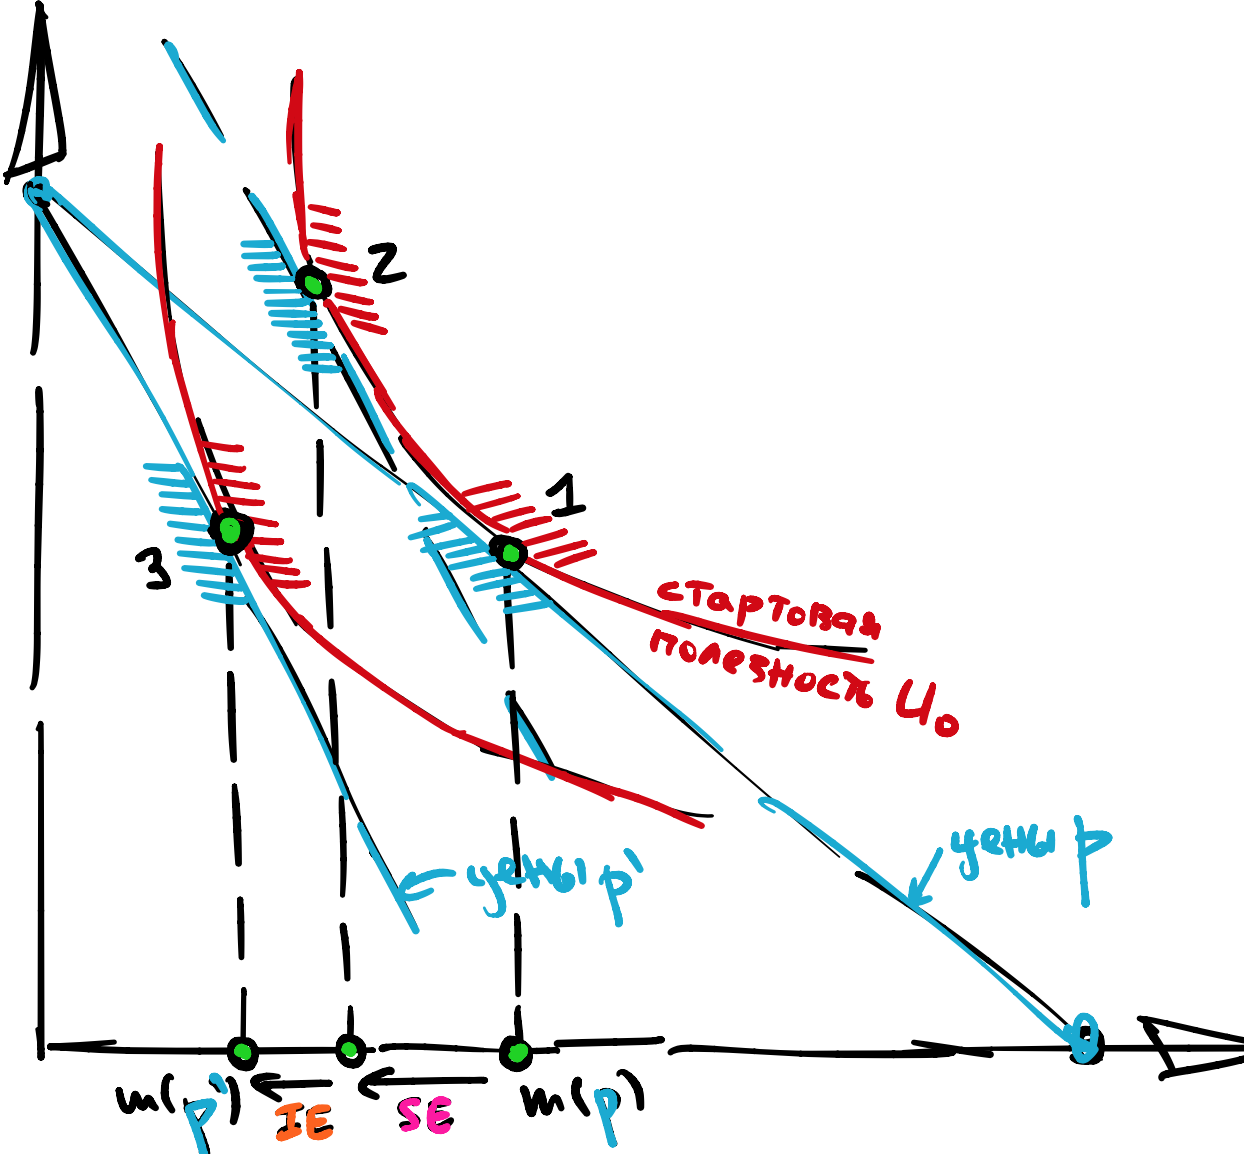
\includegraphics[width=.8 \textwidth]{./SEIETE.png}
\end{figure}

\end{frame}

\begin{frame}{Общий эффект}

Есть также общий эффект (TE), он равен сумме эффекта замещения и эффекта дохода и представляет собой просто стандартное изменение маршаллианских спросов:
$$ \text{TE} = \text{SE} + \text{IE} = m(p') - m(p).$$

Поскольку маршаллианский спрос, как правило, наблюдаем, то можно считать, что общий эффект всегда известен. Неизвестно его разложение на эффект дохода и замещения.

\end{frame}

\section{Эффект замещения}

\begin{frame}{Эффект замещения}

Эффект замещения есть, по сути, приращение хиксианского спроса при полезности зафиксированной на изначальном уровне. 
$$ SE = h(p', \bar U_0) - h(p, \bar U_0) $$

\end{frame}

\begin{frame}{Эффект замещения}

\begin{figure}[hbt]
\centering
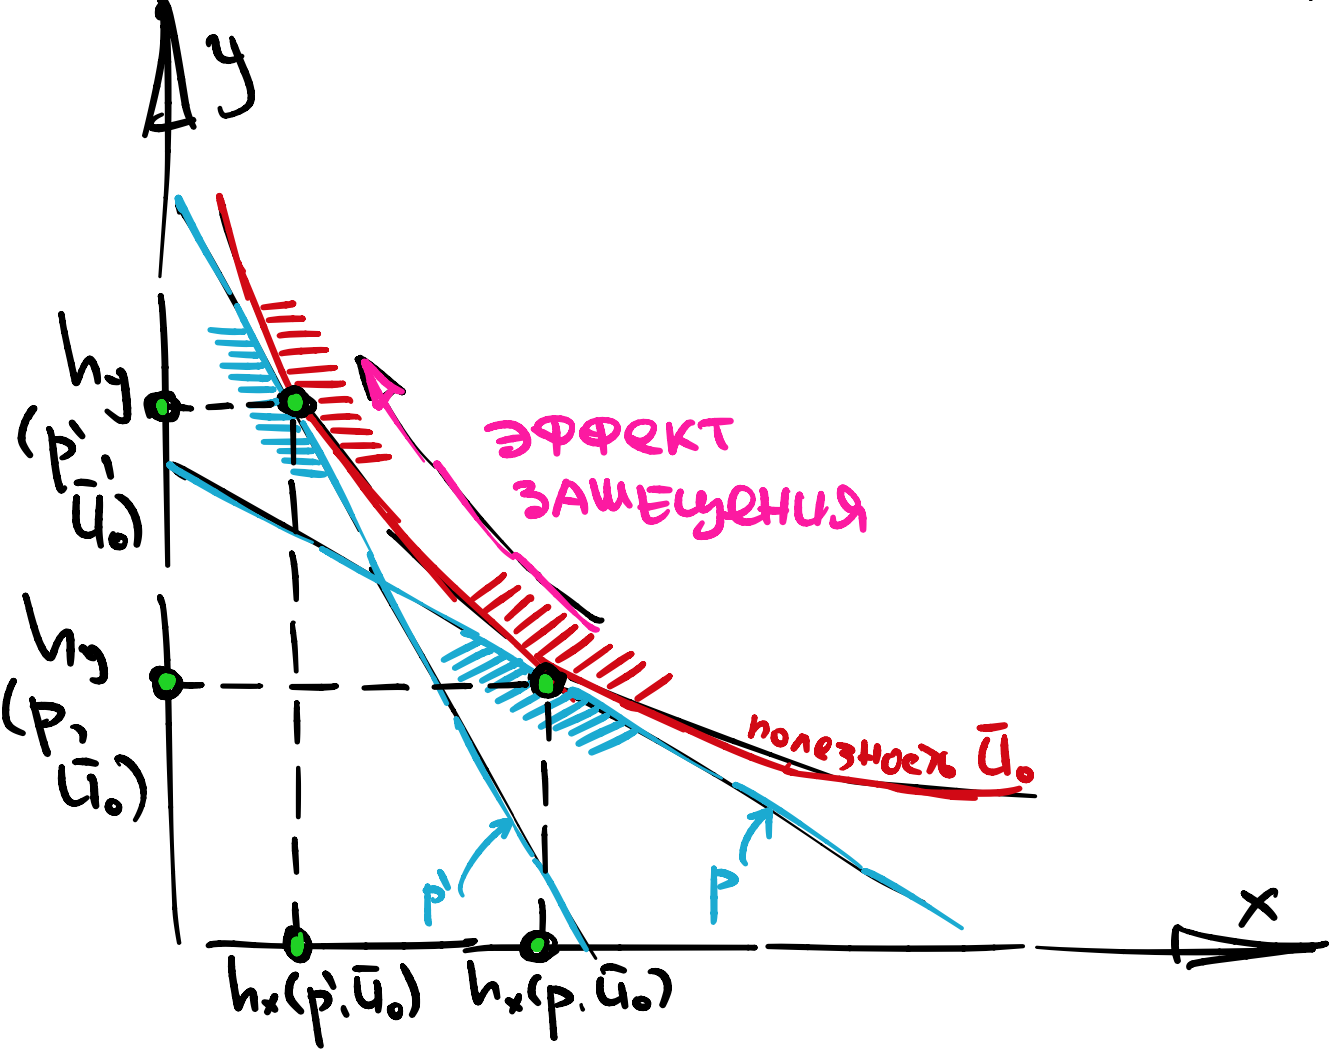
\includegraphics[width=.8 \textwidth]{SE.png}
\end{figure}

\end{frame}

\section{Эффект дохода}

\begin{frame}{Эффект дохода}

Эффект дохода есть разница между общим эффектом и эффектом замещения, именно так его надо считать. 

Однако сам по себе он не представляет большого интереса. Вообще не очень понятно, зачем вычислять кусок спроса, за который отвечает эффект дохода. 

\end{frame}


\begin{frame}{Эффект дохода}

Гораздо интереснее понять, какому изменению бюджета соответствует эффект дохода? Тогда при любом изменении цен, мы можем сказать насколько мы <<ограбили>> того или иного потребителя в рублях.

 То есть, при новых ценах $p'$, это стоимость (в рублях) возвращения агента на старый уровень полезности. Это же как раз компенсирующая вариация:
$$ CV = IE \cdot p' $$

\end{frame}

\begin{frame}{Эффект дохода}

\begin{figure}[hbt]
\centering
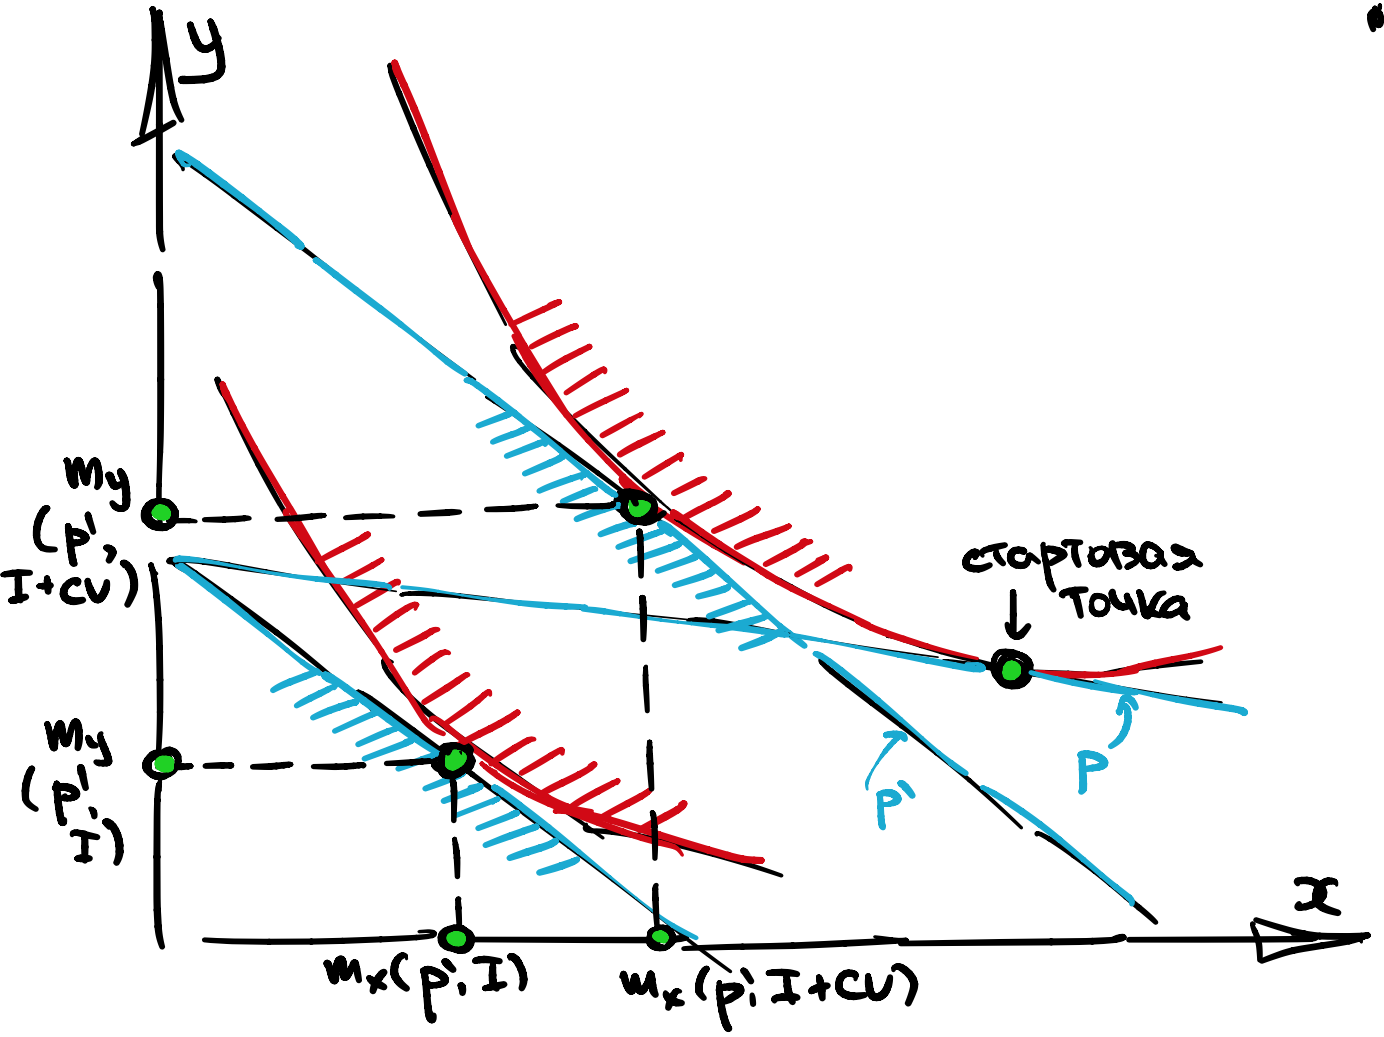
\includegraphics[width=.8 \textwidth]{IE.png}
\end{figure}

\end{frame}

\section{Парадокс Гиффена}

\begin{frame}

Парадокс Гиффена заключается в том, что для некоторых товаров, которые пользовались популярностью у бедных: картофель и дешевый хлеб – наблюдалась прямая зависимость между ценой и спросом. Похожая зависимость иногда прослеживается для спроса на рис в современном Китае.

Разрешение парадокса осуществляется за счет анализа Хиксианского спроса и матриц Слуцкого. 

\end{frame}

\begin{frame}

Обратим внимание еще раз на эластичность Хиксианского спроса по собственной цене, $\varepsilon^c_{x,p}$:
$$\varepsilon^c_{x,p} = \varepsilon_{x,p} + \varepsilon_{x,I} \cdot s_{x},$$

и перепишем ее так, чтобы маршаллианский спрос был слева:
$$\varepsilon_{x,p} = \varepsilon^c_{x,p} - \varepsilon_{x,I} \cdot s_{x}.$$

Легко видеть, что если $\varepsilon_{x,I} > 0$, то, поскольку $\varepsilon^c_{x,p}$ всегда неположительный (см. отрицательно определенные матрицы), и $\varepsilon_{x,p}$ будет неположительный. 

А нам нужна положительная зависимость между $x,p$. 
\end{frame}

\begin{frame}

Соответственно, можно сделать следующий вывод:

\alert{Нормальный товар не объяснит парадокс Гиффена.}

\end{frame}

\begin{frame}
Предположим, наоборот, что товар $x$ инфериорный, то есть это товар низкого качества, тогда $\varepsilon_{x,I} < 0$. Предположим также, что доля товара $x$ в бюджете потребителя достаточно высока, то есть $s_{x}$ большой. Наконец, предположим, что для товара $x$ нет близкого (чистого) субститута, то есть $\varepsilon^c_{x,p}$ близок к нулю.

Тогда может так случиться, что $\varepsilon_{x,p}$ станет положительным.

\end{frame}

\begin{frame}
Еще раз
$$\varepsilon_{x,p} = \varepsilon^c_{x,p} - \varepsilon_{x,I} \cdot s_{x}.$$
\begin{itemize}
\item $\varepsilon^c_{x,p}$ отражает эффектом замещения
\item $\varepsilon_{x,I} \cdot s_{x}$ отражает эффектом дохода
\end{itemize}

Для того, чтобы объяснить парадокс Гиффена, нужно иметь слабый эффект замещения и сильный эффект дохода, направленный в неочевидную сторону.

\end{frame}

\begin{frame}
\begin{figure}[hbt]
\centering
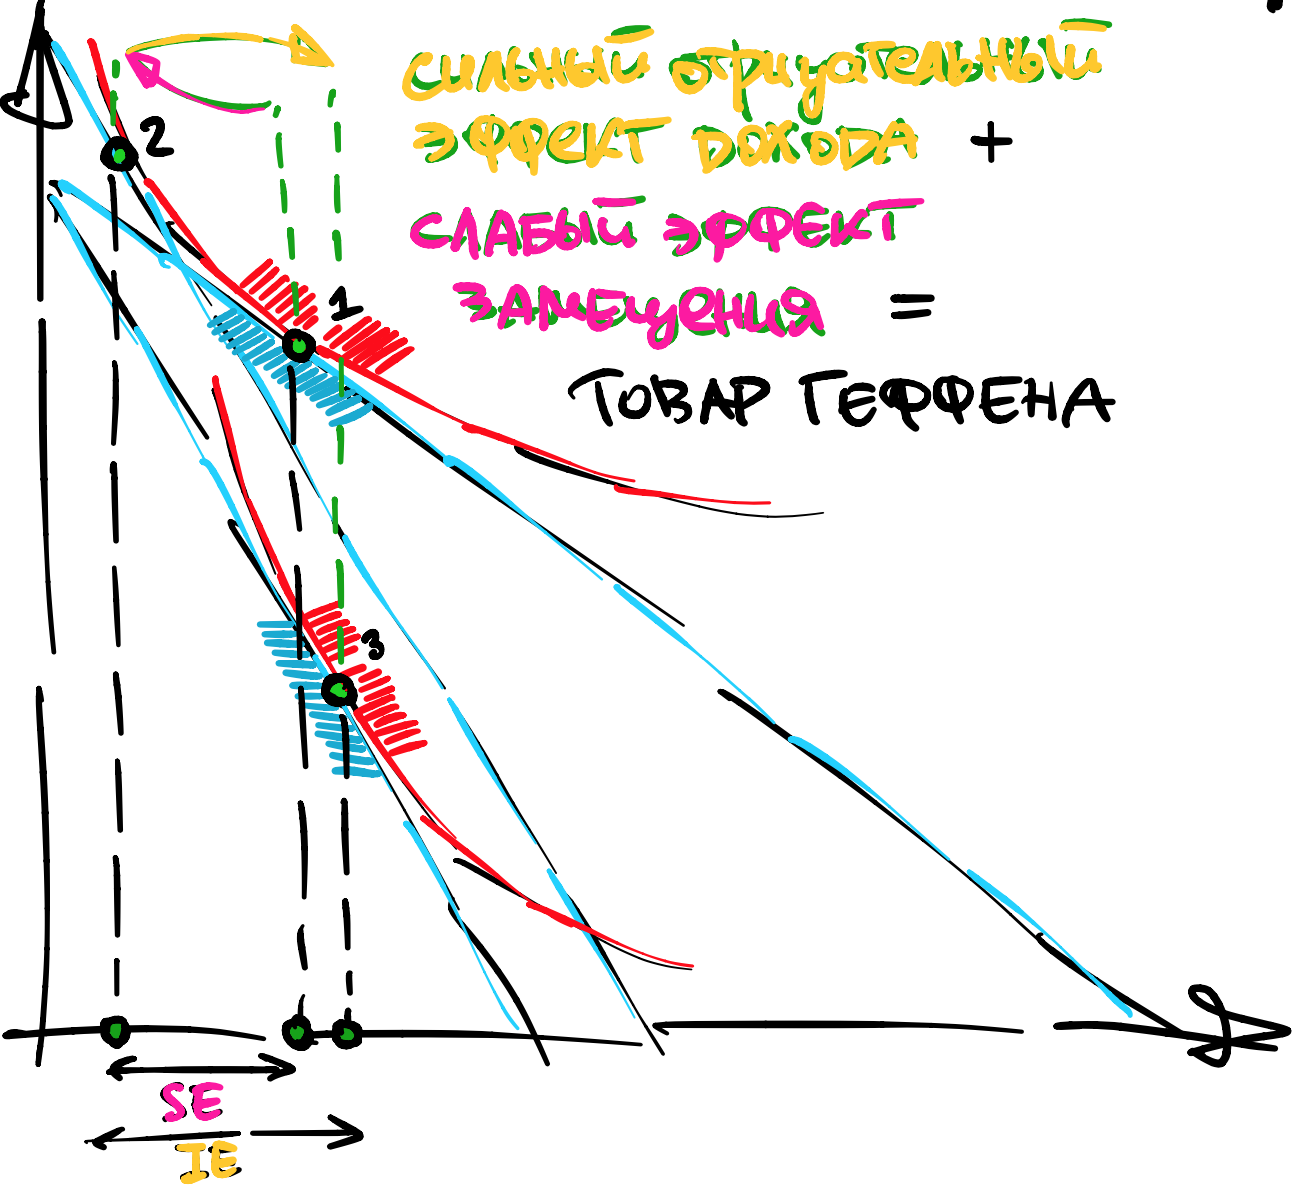
\includegraphics[width=.8 \textwidth]{IESE_CV.png}
\end{figure}

\end{frame}

\begin{frame}

Другими словами, если цена на товар который ко всему комплемент (например рис  хлеб или яичная лапша) растет, а близкого субститута нет, то вы, по факту, обеднели. Потому что вы обеднели, вы стали покупать больше этого товара (риса хлеба или яичной лапши), потому что он как раз отрицательно скорелирован с доходом (это инфериорный товар).

\alert{Три факта}:
\begin{itemize}
  \item большая доля
  \item инфериорнисть
  \item отсутствие близких субститутов
\end{itemize}

\alert{позволяют объяснить парадокс Гиффена}.

\end{frame}

\section{Потренируемся считать IE и SE с Кобб Дугласом (10 - 15 минут)}

\section{Разбор эссе (до конца лекции)}

\begin{frame}
Напомню условие (запишем на доске): 
\begin{itemize}
  \item в чем суть эксперимента
  \item почему это важно
  \item какие выводы были сделаны
  \item как это вписывается в тему первой лекции
  \item критический анализ и альт. интерпретации
\end{itemize}
И всего давалось 5 баллов.
\end{frame}

\begin{frame}{МЕ, 289 words}
\tiny
Стэнфордский зефирный эксперимент показывает насколько люди способны откладывать удовольстие ради большей награды. Эксперимент был проведён много раз в разных условиях, но во всех его вариациях \alert{испытуемым предлагалась мгновенная награда или же двойное вознаграждение, если отложить получение награды}. Особая важность исследования в том, что данный эксперимент позволяет получить данные о склонности людей ждать награды, что может положительно отразиться на успехах в их дальнейшей жизни. 
    
    Ещё одна особенность данного эксперимента - способы интерпретации данных и выводов. \alert{Поэтому выводы экспериментов довольно противоречивы, и из того, что они противоречивы, следует их возножная ошибочность}. Среди них: полнота семьи положительно влияет на способность откладывать награду; возраст влияет на способность откладывать награду; богатые были более склонны отложить награждение, так как изначальная награда для них была незначительной и они привыкли, что обещания исполняются; отсутствие размышлений о награде повышает способность откладывать удовольствие, в отличии от  сосредоточения мыслей на награде; репутация исследователей сказывается на ожиданиях людей (люди могут ожидать, что их обманут).
    
    Одни из последних выводах говорят о том, что \alert{личностные особенности, что закладываются в раннем детстве, влияют на результаты эксперимента и на жизнь испытуемых в целом}. Эксперимент -  отличный пример модели, которые рассматриваются в экономике. \alert{В данной модели у каждого испытуемого есть свои предпочтения}, а также мы строим лишь предположения о том, почему испытуемые ведут себя именно так.
    
    Эксперимент имеет ряд проблем. Например, почти ни в одном эксперименте нет акцента на мнение испытуемых о своём выборе, хотя некоторые из них проводились на довольно взрослой аудитории. Однако, помимо проблем в методике проведения эксперимента, полученные данные очень сложно точно интерпретировать, так как исследователи могут легко упустить целый ряд факторов при сборе статистики. Лишь в недавних исследованиях было сказано о том, что на результат эксперимента влияют индивидуальные особенности испытаемых (их характер, особенности воспитания, привычки), что можно считать более корректным выводом эксперимента. 
\end{frame}

\begin{frame}{МЕ, 289 words}
Моя оценка 3.5-4 баллов, потому что очень слабо привязано к теме лекции (предпочтения тут, предпочтения там) и, самое главное, нет конструктивной критики
\begin{itemize}
  \item результаты противоречивы, ок
  \item не спросили мнение, ок
  \item сложно интерпретировать, ок
\end{itemize}
Эти аргументы можно применить к абсолютно любому дизайну эксперимента. Если ты знаешь как лучше - скажи как надо было сделать. Если ты знаешь в чем ошибка - назови ее.

\end{frame}

\begin{frame}{ЛТ, 125 words}
\tiny
\alert{Суть эксперимента: детям давали выбор между моментальной наградой или более желанной наградой, но через некоторое время.} Обычно в роли награды выступали сладости.
\alert{По результатам первого эксперимента дети, которые дожидались более ценной награды показывали большие успехи в жизни, чем те, что не дожидались.}  
Затем проводились различные эксперименты, с модификациями. Результаты которых говорят о влиянии различных факторов. Например \alert{достаток семьи, в бедной семье - "завтра не наступает", в богатой - награды ничего не стоят так как дома и так много сладостей.}
Итог - интересный эксперимент, но с одной стороны безполезный, так как \alert{нельзя его результат экстраполировать, из-за множества факторов}, а с другой заставляет учитывать, что все люди разные. 
\alert{В нашу лекцию этот эксперимент вписывается тем, что нельзя сравнивать полезности различных людей} из-за множества индивидуальных факторов (дисконтирования, жизненного опыта...).

\end{frame}

\begin{frame}{ЛТ, 125 words}
Моя оценка 3 балла, потому что очень уж коротко и, опять же, нет конструктивной критики
\begin{itemize}
  \item однако, суть передана правильно
  \item определенные выводы есть
\end{itemize}
Ответ <<так как нельзя его результат экстраполировать, из-за множества факторов>>, хотя я и согласен, невозможно засчитать полностью, поскольку он не развернут. <<нельзя экстраполировать>> - это тезис, а <<множества факторов>> это его подтверждение. Соотношение тезис-подтверждение не может быть 1:1, это должно быть хотя бы 1:3 или 1:5.
\end{frame}

\begin{frame}{ГА, 237 words}
\tiny
Оригинальный Стэнфордский зефирный эксперимент, проведенный Вольтером Мишелем в 1970 году, был призван изучить, когда в детях развивается способность ждать, чтобы получить то, что они хотят. \alert{В ходе эксперимента детям разного возраста давался выбор получить сладость сейчас, или подождать пока экспериментатор вернется и получить более предпочтительную сладость.} Иследователям было важно это знать, потому что, во-первых, у них была идея, что умение терпеть ради будущего можно развивать, а во-вторых, это умение потенциально могло предсказывать некоторый успех в будующим. В 1972 году был произвеен еще один эксперимент. \alert{Общим выводом двух экспериментов стал факт, что способность детей к отсрочке удовольствия зависит от механизмов подавления мыслей о желаемом}, хотя изночально предполагалось, что чем больше думаеи о том, чего хотим, тем больше готовы терпеть. \alert{Таким образом функция полезности детей зависила не только от почуленных благ и времени ожидания, но и от условий (видели ли они сладости и тд). Но данный эксперимент имеет ряд недостатков.} Самый яркий из них это очень однородная выборка (большинство детей отпрыски профессоров или выпускников). Выборка должна быть более общирной для получения общих для человечества выводов. Также эксперимент не учитывал степень голода детей. Более того, последующее изучение жизни исследуемых с помощью опросов может дать не совсем точьные данные (лучше использовать объективные количественные данные). 
\alert{Альтернативные выводы, которые можно сделать: чтобы предсказать, возьмет ли ребенок сладость надо смотреть на благосостояние его семьи (бедные склоны не ждать), а вот будущее детей больше зависит от окружения, чем от умения или неумения ждать для получения выгод.}
\end{frame}

\begin{frame}{ГА, 237 words}
Моя оценка 4 балла, потому что хороший баланс всего\begin{itemize}
  \item суть эксперимента 1 предложение + 2 предложения деталей
  \item общие выводы 1 предложение, хотя я и не согласен
  \item очень конструктивная критика (малая, нерепрезентативная выборка)
\end{itemize}
Механизмы подавления не следуют из текста эссе. Более того, в эссе отсутствует упоминание о том, что дети не выбравшие зефирку добились лучших результатов 40 лет спустя. То есть, стилистически все хорошо, но видно что человек не до конца разобрался.
\end{frame}

\begin{frame}{ГК, 290 words}
\tiny
Зефирный эксперимент Стэндфордского университета является достаточно известным кейсом. \alert{Его основная суть заключается в исследовании поведения детей дошкольного возраста в ситуации выбора между получением одной зефирки сейчас или нескольких потом (в зависимости от даты проведения награды варьировались, но суть оставалась та же, либо что-то сейчас, либо что-то лучше через 15 минут).} 
\alert{Данный эксперимент является важным, потому что на примере маленьких детей (только начинающих процесс образования и социализации, не знающих про рациональное поведение экономического агента и т.д.) проверяет базовую поведенческую модель выбора, то есть показывает насколько человек по-сути на биологическом уровне способен рационально или нерационально мыслить и действовать.} Отдельный интерес вызывают результаты исследования, показавшие, что в дальнейшем по жизни дети, которые дольше ждали награду становились успешнее по основным показателям в жизни. В частности лучше писать SAT и в целом были лучше в образовании. И несмотря на то, что последующие исследования частично опровергли данное предположение, подтвердив, что на способность ждать большей награды влияют различные внешние факторы, такие как экономический бэкграунд семьи из которой произошёл ребёнок или то, обманывали ли ребёнка раньше в подобных ситуациях, всё же изначальный итог эксперимента по праву остаётся актуальным. То есть было доказано очевидное влияние других факторов, однако базовый тезис полностью опровергнут не был.
\alert{В контексте темы первой лекции интерес представляет одна из вариаций эксперимента, в котором симулировали разные кондиции и влияние различных отвлекающих факторов на исход эксперимента.} Этот эксперимент показал, что эффект при котором ребёнок дольше ждёт наступает не в результате просто мыслей о чём-то другом, а в результате комплексных механизмов избегания мыслей о награде, полного переключения на что-то другое. \alert{Например: часть наиболее успешных в ожидании детей пели песни, играли со своими пальцами, несколько детей и вовсе заснули.} То есть у них расширился выбор, помимо ожидания награды они смогли найти себе другие занятия и это привело к успеху. 
\end{frame}

\begin{frame}{ГА, 290 words}
Моя оценка 4.5-5 баллов, потому что хороший баланс всего и глубокий анализ
\begin{itemize}
  \item лучше всего отвечать на вопрос с самого вопроса: суть эксперимента в том что... эксперимент важен потому что... и так далее
  \item Первое предложение - трата квоты слов
  \item Немного уклон в нейропсихолоогию (песни и игра с пальцами), но тем не менее неожиданно успешно связано с темой лекции (множество альтернатив)
\end{itemize}

Связь выводов и критика не совсем то что я ожидал, но, в контексте эссе выглядит цельно и законченно.

\end{frame}

\section{Конец}

\end{document}